%!TEX root = ../dokumentation.tex

\chapter{Implementierung der Knoten}

Mit BaklavaJS wurde das Grundgerüst der Applikation erstellt. Auf BaklavaJS aufbauend wird im \ac{MLTDG} die Funktionalität mittels der verschiedenen Knoten implementiert. In diesem Kapitel wird zum einen vorgestellt, welche Knoten implementiert wurden. Zum anderen wird darauf eingegangen, wie die grafische Oberfläche für einstellbare Wahrscheinlichkeitsverteilungen implementiert wurde.

\section{Knoten-Arten}
Der Kern der Applikation bilden die verschiedenen Knoten: Mit ihnen kann das Modell aufgebaut werden. Dabei ist es wichtig, dass die Knoten die verschiedenen Anwendungsfälle abdecken.

Um herauszufinden, welche Knoten-Arten benötigt werden, wurden mehrere Beispiel-Modelle durchgespielt und evaluiert, mit welchen Knoten diese sich am besten umsetzen lassen. Beispielhaft ist hier ein Modell dargestellt, welches Daten für einen fiktiven Immobilienmarkt generieren kann:
\begin{algorithm}[H]
    \caption{Beispielmodell Immobilienmarkt}
    \begin{algorithmic}[1]
        \State Fläche = ZufallGauss($\mu = 80$, $\sigma = 20$)
        \State a = Mathematik(Division, $\textrm{Fläche}$, $40$)
        \State b = ZufallDiskret($-1: 10\%, 0: 80\%, 1: 10\%$)
        \State c = Mathematik(Addition, $a$, $b$)
        \State Räume = Mathematik(Maximum, $c$, $1$)
        \State d = $\textrm{Fläche} \cdot 2500 + 250 \cdot \textrm{Räume}$
        \State Preis = ZufallProzentual($d$, $5\%$)
    \end{algorithmic}
\end{algorithm}

Die Knoten lassen sich in folgende Kategorien unterteilen:
\begin{itemize}
    \item \textbf{Werteknoten} können benutzt werden, um den gleichen Wert an verschiedene andere Knoten weiterzugeben. Es gibt sie für die Datentypen \textit{Boolean}, \textit{Number} und \textit{String}. Zusätzlich gibt es den Index-Knoten. Dieser gibt den aktuellen Index innerhalb des Berechnungsprozesses aus. Wird ein Wert nur für einen Knoten verwendet, kann dieser in der Regel direkt an der Eingangsschnittstelle des entsprechenden Knotens eingestellt werden; ein Werteknoten muss dafür nicht verwendet werden.
    \item \textbf{Zufallsknoten}
    \begin{itemize}
        \item \textbf{Gleichverteilung} mit einstellbarem Minimum und Maximum
        \item \textbf{Normalverteilung} mit einstellbarem Mittelwert $\mu$ und Standardabweichung\nobreakspace $\sigma$
        \item \textbf{Exponentialverteilung} mit einstellbarem $\lambda$
        \item \textbf{Anpassbare Verteilung}: Bei diesem Knoten kann die Wahrscheinlichkeitsdichtefunktion über einen grafischen Editor eingestellt werden. Die Wahrscheinlichkeitsdichtefunktion kann sowohl diskret als auch stetig sein.
        \item \textbf{Prozentuale Abweichung}: Dieser Knoten nimmt einen Wert und addiert einen zufälligen Wert zwischen $\pm \, \, inputValue \cdot \frac{percentage}{100}$
    \end{itemize}
    \item \textbf{Berechnungsknoten}
    \begin{itemize}
        \item \textbf{Mathematik}: Der Mathematikknoten wendet eine einstellbare mathematische Funktion, wie zum Beispiel Addition, Division oder trigonometrische Funktionen auf ein oder zwei Eingabedaten an
        \item \textbf{Funktion}: Der Funktionsknoten kann benutzt werden, um eine beliebige Funktion in JavaScript zu implementieren. Alle Eingangswerte werden im \texttt{this} Objekt zur Verfügung gestellt. Der Code muss ein Objekt zurückgeben, welches die Namen der Ausgangsschnittstellen als Keys und die dazugehörigen Werte enthält.
        \item \textbf{Boolean}: Dieser Knoten vergleicht zwei numerische Werte und gibt das Resultat des Vergleichs aus.
        \item \textbf{Stringlist}: Der Stringlist-Knoten erlaubt es, einen String aus einer vorgegebenen Liste von Strings auszuwählen. Welcher String ausgegeben wird, kann über die Index-Eingangsschnittstelle gesteuert werden (die Indizes beginnen bei 0)
    \end{itemize}
    \item \textbf{Bedingungsknoten}: Bedingungsknoten können genutzt werden, um sicherzustellen, dass Ausgabedaten bestimmte Bedingungen erfüllen. Wenn an der Eingangsschnittstelle der Wert \texttt{false} anliegt, wird der aktuelle Datenpunkt neu berechnet.
    \item \textbf{Ausgabeknoten}: Jeder Ausgabeknoten repräsentiert eine Spalte in den generierten Ausgabedaten. Der Name der Spalte kann im Textfeld des Ausgabeknotens gesetzt werden.
\end{itemize}

\section{Anpassbare Verteilung}
\label{sec:anpassbareverteilung}

Besteht die Aufgabe Daten zu generieren, die von Zufallswerten einer komplexen Wahrscheinlichkeitsverteilung abhängen, gibt es das Problem, dass mit standardmäßigen Verteilungen oft keine passende Wahrscheinlichkeitsverteilung gefunden werden kann. Beispielsweise könnte eine Wahrscheinlichkeitsverteilung mit folgenden Anforderungen verlangt sein:
\begin{itemize}
    \item Hochpunkte an den Stellen $1$, $4$ und $9$
    \item Keine Generation von Werten zwischen $5$ und $7$
\end{itemize}
Solch eine Wahrscheinlichkeitsverteilung könnte nicht mit einer standardmäßigen Verteilung dargestellt werden. In diesem Fall soll der Benutzer in der Lage sein, schnell und einfach mit einer grafischen Oberfläche eine gewünschte Wahrscheinlichkeitsverteilung, wie in Abbildung \ref{fig:customnodeexample}, grafisch modellieren zu können.
\begin{figure}[H]
    \centering
    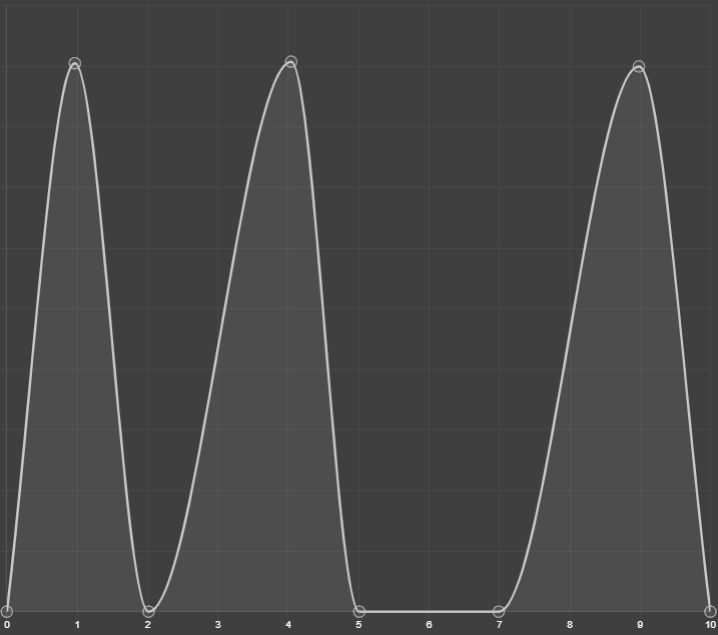
\includegraphics[width=.55\textwidth]{custom_node_example.png}
    \caption{Beispielhafte Wahrscheinlichkeitsverteilung}
    \label{fig:customnodeexample}
\end{figure}
Dadurch wird zum einen eine konzeptuelle Umgebung geschaffen, als auch der Aufwand erspart eine exakte Dichtefunktion der Wahrscheinlichkeitsverteilung zu entwerfen. Selbst wenn es keine exakte Dichtefunktion für die Wahrscheinlichkeitsverteilung gibt, könnte sie mit diesem Knoten näherungsweise modelliert werden. 

Da die grafische Modellierung einer Wahrscheinlichkeitsverteilung mit den anpassbaren Zufallsknoten im Vergleich zu den anderen Knoten deutlich höheren Implementierungsaufwand benötigt, wird auf deren Umsetzung näher eingegangen. Die folgenden Kapiteln behandeln die grafische Modellierung von stetigen und diskreten Wahrscheinlichkeitsverteilungen. Wie dann tatsächlich aus der  modellierten Wahrscheinlichkeitsverteilung eine Zufallszahl generiert werden kann, wird in Kapitel \ref{sec:anpassbareverteilungberechnung} (S. \pageref{sec:anpassbareverteilungberechnung}) erklärt.

\subsection{Bibliothek zur Darstellung von Wahrscheinlichkeitsverteilungen}

Je nachdem, ob eine stetige oder diskrete Wahrscheinlichkeitsverteilung visualisiert werden soll, unterscheidet sich auch die Diagrammart. Ein Verteilungsdiagramm für stetige Werte wird mit einer Kurve modelliert. Hingegen wird für diskrete Werte ein Säulendiagramm verwendet. 

Für die grafische Oberfläche der beiden Knoten wird ein freier Zeichenraum benötigt, auf dem das Linien- oder Säulendiagramm gezeichnet werden kann. Zudem soll die Oberfläche Interaktionsmöglichkeiten zur Gestaltung der Verteilung geben. Da es bereits einige Implementierungen von Visualisierungsmöglichkeiten in JavaScript gibt, wird an dieser Stelle auf eine bereits existierende Lösung zurückgegriffen. Hierfür wird das JavaScript Framework Chart.js verwendet \cite{chartjs}. Dies hat folgende Gründe:
\begin{itemize}
    \item Open-Source mit MIT License: Freie Nutzung ohne anfallende Kosten
    \item Unterstützung von 8 Chart-Typen: Inklusive Linien- und Säulendiagramm
    \item HTML5 Canvas: Hohe Rendering-Leistung
    \item Responsive: Diagramme werden in einer skalierbaren Sidebar verwendet
\end{itemize}

\subsection{Grafische Modellierung einer stetigen Wahrscheinlichkeitsverteilung}

Für die stetige Wahrscheinlichkeitsverteilung müssen in dem Liniendiagramm Interaktionsmöglichkeiten zum Hinzufügen (Doppelklick), Löschen (Rechtsklick) und Verschieben (Linkslick) von Punkten implementiert werden. Die Punkte sind durch eine Linie miteinander verbunden. Im linearen Modus werden zwei aufeinanderfolgende Punkte mit einer Geraden verbunden (vgl. Abb. \ref{fig:customnodelinear}).

\begin{figure}[H]
    \centering
    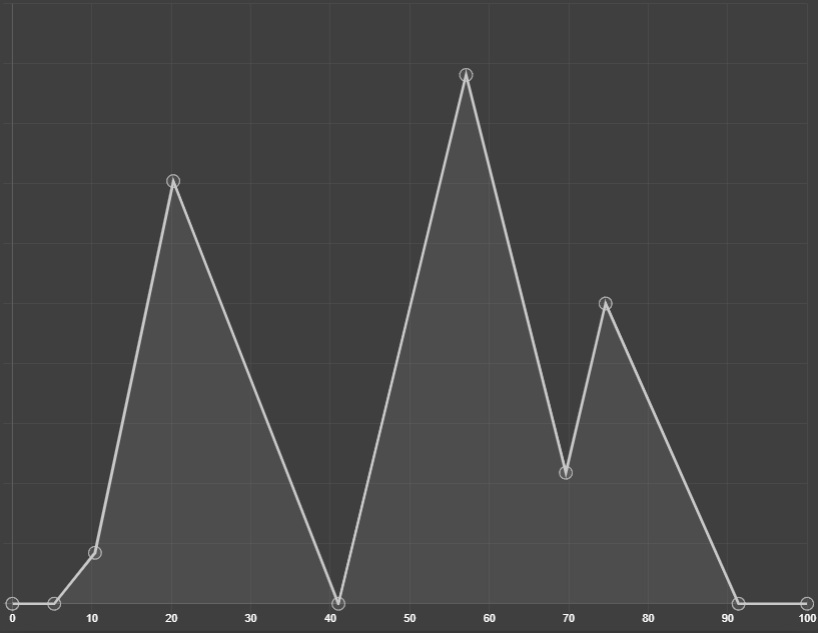
\includegraphics[width=.55\textwidth]{custom_node_linear.png}
    \caption{Grafische Oberfläche einer stetigen Wahrscheinlichkeitsverteilung im linearen Modus}
    \label{fig:customnodelinear}
\end{figure}

Oft ist ein linearer Zusammenhang nicht realistisch genug, um eine Wahrscheinlichkeitsverteilung zu beschreiben. Um gekrümmte Verbindungen zwischen den Punkten zu erstellen, kann eine sogenannte Spline-Interpolation verwendet werden. Chart.js bietet bereits Interpolationsmöglichkeiten, die für die Visualisierung eingesetzt werden können, jedoch gibt es keine geeignete Schnittstelle, um auf die Interpolationsdaten zuzugreifen. Ein Spline-Algorithmus muss deshalb selbst implementiert werden. Die genaue Spline-Funktion wird zwingend benötigt, um die Werte zwischen den erstellten Punkten berechnen zu können.

Es gibt mehrere Vorgehensweisen, um passende Splinefunktionen zu finden. 
Kubische Splines interpolieren eine Menge von Kontrollpunkten mit Hilfe von
stückweisen kubischen Polynomen. Die Verwendung von Polynomen niederer Ordnung ist für die Kurvenanpassung besonders attraktiv, da sie sehr performant sind und numerische Instabilitäten verhindern, die bei höhergradigen Kurven entstehen können. Diese Instabilitäten verursachen ein unpassendes Kurvenverhalten. Höhergradige Funktionen sind oft zu aufwändig bei der Berechnung, um sie für Interpolationszwecke einzusetzen. Das wohl überzeugendste
Argument der kubisch hermiteschen Interpolation ist aber ihre $C^2$-
Kontinuität, die garantiert, dass sich die Splinefunktion kontinuierlich über die erste und zweite Ableitung aller Polynomsegmente fortsetzt.
Kontinuität erzwingt einen glatte Transition über die ganze Kurve hinweg. \cite{Wolberg1999}

Die Splinefunktion soll so bestimmt werden können, dass die gewünschte Wahrscheinlichkeitsverteilung am einfachsten und intuitivsten erstellt werden kann. Die kurvenartige Struktur von Splines ermöglicht es zwar, realistische beziehungsweise glatte Kurven zu erstellen. Jedoch haben die meisten Splines eine Tendenz zu überschwingen. 

Überschwingen ist die Bezeichnung für eine sprunghafte Änderung, wodurch eine Funktion über den eigentlich angezielten Wert hinausschießt und sich erst im weiteren Verlauf dem eigentlichen Wert annähert. Leider neigen kubisch hermitesche Splines zu diesem Überschwingen, weshalb ihre Nutzung in dieser Form für die Applikatoin ungünstig ist. \cite{kruger:2007}

\begin{figure}[H]
    \center
    \begin{tikzpicture}
        \begin{axis}[
            xmin=0,
            xmax=3,
            ymin=0,
            ymax=10
        ]
        \addplot[
            mark=*,
            patch,
            red,
            patch type=cubic spline,
            thick,
        ]
        coordinates {
            % left, right, left middle, right middle
            (0,1) 
            (3,9)
            (1,6)  
            (2,2)
        };
        \end{axis}
    \end{tikzpicture}
    \caption{Spline mit Überschwingen}\label{fig:spline}
\end{figure}

In Abbildung \ref{fig:spline} ist ein kubisch hermitescher Spline zu erkennen, der zwischen den vier Kontrollpunkten $P_1(0,1)$, $P_2(1,6)$, $P_3(2,2)$ und $P_4(3,9)$ interpoliert. Es ist deutlich zu erkennen, wie das Splinepolynom zwischen $P_1$ und $P_2$ über den y-Wert von $P_2$ überschwingt. Auch zwischen $P_3$ und $P_4$ ist ein Unterschwingen zu erkennen.

Um das Über- und Unterschwingen zu verhindern, muss die Monotonie-Eigenschaft der Splinefunktion garantiert werden.

\begin{figure}[H]
    \center
    \begin{tikzpicture}
        \begin{axis}[
            xmin=0,
            xmax=3,
            ymin=0,
            ymax=10]
        ]
        \addplot+[smooth] coordinates {
            (0,1) 
            (1,6)  
            (2,2)
            (3,9)
        };
        \end{axis}
    \end{tikzpicture}
    \caption{Monotone Kubische Interpolation}\label{fig:monotonespline}
\end{figure}

In Abbildung \ref{fig:monotonespline} ist ein monotoner kubischer hermitescher Spline gezeichnet mit identischen Kontrollpunkten zu Abbildung \ref{fig:spline}. Bei dieser Splinefunktion ist der Monotoniecharakter dadurch zu erkennen, dass sowohl das Überschwingen, als auch das Unterschwingen verhindert wird, was ein intuitiveres Kurvenverhalten fördert. Das Über- und Unterschwingen wird vor allem dann deutlich, wenn beide Kurven überlagert werden (vgl. Abb. \ref{fig:diffmonotone}).

\begin{figure}[H]
    \center
    \begin{tikzpicture}
        \begin{axis}[
            xmin=0,
            xmax=3,
            ymin=0,
            ymax=10
        ]
        \addplot[
            mark=*,
            patch,
            red,
            patch type=cubic spline,
            thick,
        ]
        coordinates {
            % left, right, left middle, right middle
            (0,1) 
            (3,9)
            (1,6)  
            (2,2)
        };

        \addplot+[
            smooth,
            blue
        ] 
        coordinates {
            (0,1) 
            (1,6)  
            (2,2)
            (3,9)
        };
        \end{axis}
    \end{tikzpicture}
    \caption{Hermitescher Spline vs. Monotoner Spline}\label{fig:diffmonotone}
\end{figure}

Eine sehr einfache Art Punkte monoton kubisch zu interpolieren erarbeiten Fritsch und Carlson in ihrem Paper von 1980. Sie stellen notwendige und ausreichende Bedingungen für die Monotonie der Spline-Polynome auf. Der Fritsch-Carlson-Algorithmus führt eine einfache erste Schätzung der Tangentensteigungen durch und übergibt dann erneut Datenpunkte, um eventuell überschwingende Tangenten in die monotone Region zu verschieben \cite{Fritschcarlson:1980}. Es gibt andere Algorithmen, wie zum Beispiel die Fritsch-Butland-Methode, die aufwändigere erste Schätzungen von Tangenten macht, sodass die Tangenten garantiert im monotonen Bereich liegen und kein zweiter Durchgang erforderlich ist \cite{Fritschbutland:1984}.

Da sich die Fritsch-Carlson-Methode vergleichsweise schnell und einfach implementieren lässt, wird sie für die monotone kubische Interpolation verwendet. Die Fritsch-Carlson-Methode beschreibt einen Weg um interpolierende Tangentensteigungen für jeden Kontrollpunkt so zu wählen, dass alle Splinesegmente monoton bleiben. Wie bereits erwähnt benötigt die Methode zwei Durchläufe. 

Seien die Kontrollpunkte gegeben durch $P_i(x_i,y_i)$ für $1\le i \le n$.
Im ersten Durchlauf wird für den ersten bis vorletzten Kontrollpunkt, das heißt für $i=1,\dots,n-1$, die Steigung zum darauffolgenden Kontrollpunkt berechnet mit 
$$delta_i=\frac{y_{i+1}-y_i}{x_{i+1}-x_i}$$
Die vorläufige Tangentensteigung für alle Kontrollpunkte bis auf die Randknoten, das heißt für $i=2,\dots,n-1$, ist dann bestimmt als der Median der beiden Steigungen zum vorherigen und folgenden Kontrollpunkt.
$$m_i=\frac{delta_{i-1}+delta_i}{2}$$
Wenn es ein Vorzeichenwechsel bei den Steigungen gibt, dann ist der Kontrollpunkt $P_i$ ein lokales Extremum. In diesem Fall muss die Steigung an der Stelle $x_i$ auf $0$ gesetzt werden, das heißt
$m_i=0$, wenn $delta_i\cdot delta_{i-1} < 0$.
Die Randwerte sind hierbei durch ihre einseitigen Differenzen bestimmt:
$m_1=delta_1$, $m_{n}=delta_{n-1}$.

Im zweiten Durchlauf werden die Tangentensteigungen hinreichend geprüft und korrigiert. Zunächst werden alle Sattelbereiche gefunden und die Steigungen auf $0$ gesetzt. Ein Sattelbereich ist bei einer Funktion dann vorhanden, wenn zwei aufeinanderfolgende Punkte $P_i$, $P_{i+1}$ den gleichen y-Wert haben $y_i=y_{i+1}$ für $i=1,\dots,n-1$. Da aber bereits die Sekantensteigungen berechnet worden sind, kann auch überprüft werden, ob die Sekantensteigung gleich $0$ ist, das heißt $m_i=m_{i+1}=0$, wenn $delta_i=0$. Für alle restlichen Steigungen haben Fritsch und Carlson herausgefunden, dass die Splines dann monoton sind, wenn alle Tangenten in einem bestimmten Bereich der Alpha-Beta-Ebene liegen.
Alpha und Beta sind hierbeit wie folgt definiert: 
$$\alpha_i =\frac{m_i}{delta_i}, \beta_i =\frac{m_{i+1}}{delta_i}$$
Eine robuste Wahl ist es, Alpha und Beta in einen Kreis mit Radius 3 zu setzen.
$$m_i=\tau_i\alpha_i delta_i, m_{i+1}=\tau_i\beta_i delta_i$$ mit $\tau_i=\frac{3}{\sqrt{\alpha_i^2+\beta_i^2}}$, wenn $\alpha^2+\beta^2>9$. \cite{Fritschcarlson:1980}

In dem folgenden Listing \ref{Fritsch-Carlson} wird in vereinfachter Form beispielhaft der Fritsch-Carlson-Algorithmus in JavaScript implementiert.
\begin{lstlisting}[caption=Fritsch-Carlson Methode,label=Fritsch-Carlson]
    fritschCarlson(xs, ys) {
        const delta = [];
        const ms = [];
        const n = xs.length;
        for (let i = 0; i < n - 1; i++) {
            delta[i] = (ys[i + 1] - ys[i]) / (xs[i + 1] - xs[i]);
            if (i == 0) {
                continue;
            }
            if (delta[i] * delta[i - 1] < 0) {
                ms[i] = 0;
            } else {
                ms[i] = (delta[i - 1] + delta[i]) / 2;
            }
        }
        ms[0] = delta[0];
        ms[n - 1] = delta[n - 2];
        for (let i = 0; i < n - 1; i++) {
            if (delta[i] === 0) {
                ms[i] = 0;
                ms[i + 1] = 0;
            } else {
                const alpha = ms[i] / delta[i];
                const beta = ms[i + 1] / delta[i];
                const dist = Math.pow(alpha, 2) + Math.pow(beta, 2);
                const tau = 3 / Math.sqrt(dist);
                if (dist > 9) {
                    ms[i] = tau * alpha * delta[i];
                    ms[i + 1] = tau * beta * delta[i];
                }
            }
        }
        return ms;
    }
\end{lstlisting}

Zur Interpolation der Splinefunktion wird das kubische hermitesche Interpolationspolynom benötigt. Zunächst muss dafür das zu dem x-Wert passende Polynom gesucht werden. Da die berechneten Steigungen aus dem Fritsch-Carlson-Algorithmus in sortierter Reihenfolge vorliegen, kann eine binäre Suche verwendet werden. Ist das richtige Polynom $p$ gefunden, ist die Interpolation an der Stelle $t$ durch das Polynom
$$p_i(t)=(2t^3-3t^2+1)p_i+(t^3-2t^2+t)m_i+(-2t^3+3t^2)p_{i+1}+(t^3-t^2)m_{i+1}$$
definiert \cite{Pat:2009}.

Im monoton interpolierten Modus sind aufeinanderfolgende Punkte mit einem kurvigen Graphen verbunden, wodurch oft realistischere Wahrscheinlichkeitsverteilungen modelliert werden können. Das Endresultat wird in Abbildung \ref{fig:customnodemonotone} dargestellt.

\begin{figure}[H]
    \centering
    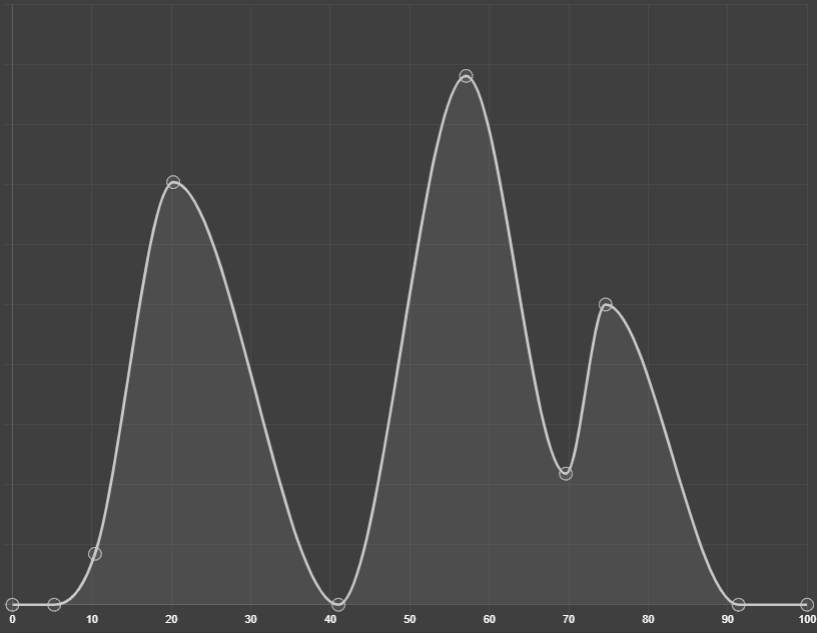
\includegraphics[width=.55\textwidth]{custom_node_monotone.png}
    \caption{Grafische Oberfläche einer stetigen Wahrscheinlichkeitsverteilung im monoton interpolierten Modus}
    \label{fig:customnodemonotone}
\end{figure}

\subsection{Grafische Modellierung einer diskreten Wahrscheinlichkeitsverteilung}

Das Säulendiagramm für die diskrete Wahrscheinlichkeitsverteilung soll dem Nutzer die Möglichkeit geben, einzelne Säulenhöhen zu setzen (Linksklick). Ein wichtiges Detail beim Setzen der Säulenhöhen ist, dass dies auch funktionieren soll, wenn der Mauszeiger sich bei gehaltener linker Maustaste über mehrere Säulen bewegt, weil sonst die Gestaltung des Verteilungsdiagramms bei einem großen Wertebereich sehr aufwändig wird. 

\begin{figure}[H]
    \center
    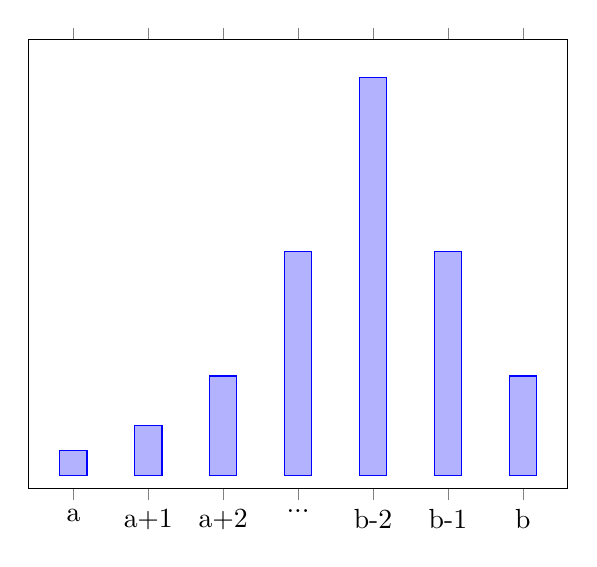
\begin{tikzpicture}
        \begin{axis}[
                ybar, 
                ytick=\empty,
                symbolic x coords={a,a+1,a+2,...,b-2,b-1,b},
            ]
            \addplot plot coordinates
                {(a,1) (a+1,2) (a+2,4) (...,9) (b-2,16) (b-1,9) (b,4)};
        \end{axis}
    \end{tikzpicture}
    \caption{Darstellung einer diskreten Verteilung}
\end{figure}

Sei der Wertebereich definiert durch die Werte $a,a+1,a+2,\dots,b-2,b-1,b$ im Intervall $[a,b]$, wobei $a,b \in\mathbb{Z}$, $x_0 \le x_n$, dann werden genau $|a-b|+1$ Klicks benötigt, wenn alle Säulen gesetzt werden sollen. Der Aufwand kann erheblich reduziert werden, indem im Optimalfall mit einem einzigen haltenden Klick und einer Bewegung der Maus alle Säulen gesetzt werden können.

Ein Problem bei dieser Funktion ist, dass oft nicht alle Säulen auf die Zeigerposition gesetzt werden, weil das mouseover-Event nicht oft genug auslöst. Dies wird durch mehrere Faktoren negativ beeinflusst:
\begin{itemize}
    \item Niedrige Skalierung des Diagramms
    \item Hohe Zeigergeschwindgkeit in horizontaler Richtung
    \item Großes Intervall $[a,b]$
 \end{itemize}

Um diesem Effekt entgegenzuwirken, kann eine Schätzung der Mausbewegung mithilfe einer linearen Interpolation vorgenommen werden. Dazu muss bei jedem Handleraufruf für das mouseDown-Event die aktuelle Position des Zeigers gespeichert werden. Der Handler für das mouseMove-Event hat dann immer die Koordinaten für die letzte und aktuelle Position des Zeigers. Seien die beiden Punkte $A(a_x|a_y), B(b_x|b_y)$ gegeben, dann ist die lineare Interpolationsfunktion für alle diskreten Werte im Intervall $[a_x,b_x]$ definiert als $f(x)=mx+a_y-m*a_x$ mit $m=\frac{b_y-a_y}{b_x-a_x}$. Alle Säulen zwischen der letzten bekannten und der aktuellen Zeigerposition können nun gesetzt werden, sodass keine Lücken mehr beim Editieren der diskreten Wahrscheinlichkeitsverteilung auftreten (vgl. Abb. \ref{fig:discretenode}).

\begin{figure}[H]
    \centering
    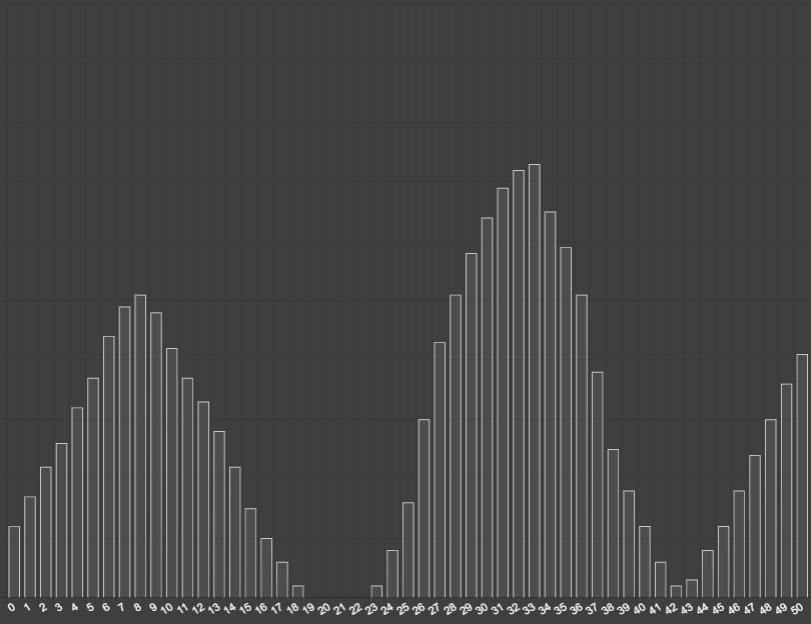
\includegraphics[width=.55\textwidth]{discrete_node.png}
    \caption{Grafische Oberfläche einer diskreten Wahrscheinlichkeitsverteilung}
    \label{fig:discretenode}
\end{figure}